%!TEX ROOT=formularioFisica.tex

\section{Cinematica}\label{sec:cinematica}
La cinematica, definita anche \emph{geometria del movimento}, si occupa dello studio dei moti. Un 
oggetto è in moto se la sua posizione cambia nel tempo. Esistono tanti modi di spostarsi: lungo una
retta, in curva, oscillando avanti e indietro attorno ad un punto. In tutti i problemi verrà 
ignorato l'attrito con l'aria.\\
Per gli esercizi si vada a pagina~\pageref{ex:cinematica}.\\[\baselineskip]
Si noti e ricordi che
\begin{equation*}
1\,\text{m/s} = 3.6\,\text{km/h}
\end{equation*}

\subsection{Moto Rettilineo Uniforme}\label{subsec:cinematica:mru}
\begin{equation*}
x = x_0 + vt
\end{equation*}
$x$: posizione finale dell'oggetto\\
$x_0$: posizione iniziale dell'oggetto\\
$v$: velocità\\
$t$: tempo

\subsection{Moto Rettilineo Uniformemente Accelerato}
\begin{equation*}
v = v_0 + at
\end{equation*}
\begin{equation*}
x = x_0 + v_0t + \frac{1}{2}at^2
\end{equation*}
\begin{equation*}
v^2 = v_0^2 + 2a\cdot\Delta x
\end{equation*}
$v$: velocità finale\\
$v_0$: velocità iniziale\\
$a$: accelerazione\\
$t$: tempo\\
$x$: posizione finale\\
$x_0$: posizione iniziale\\
$\Delta x$: $x - x_0$
\subsection{Moto Parabolico}\label{subsec:cinematica:mp}
\begin{center}
	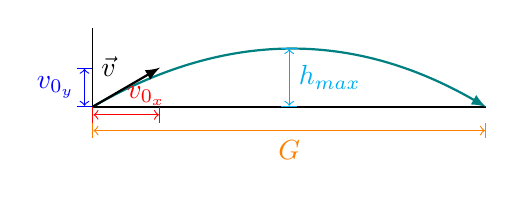
\begin{tikzpicture}
		\draw[thin] (0,0) -- (5,0);
		\draw[thin] (0,0) -- (0,1);
		\draw[-latex, teal, thick] (0,0) to[out=30, in=150] (5,0);
		
		\draw[|<->|, orange] (0, -0.3) -- (5, -0.3)
			node[pos=0.5, below]{$G$};
		\draw[|<->|, cyan] (2.5, 0) -- (2.5, 0.75)
			node[pos=0.5, right]{$h_{max}$};
		\draw[-latex, thick] (0,0) -- (0.86, 0.5)
			node[pos=0.5, above left]{$\vec{v}$};
		\draw[|<->|, red] (0,-0.1) -- (0.86, -0.1)
			node[pos=0.8, above]{$v_{0_x}$};
		\draw[|<->|, blue] (-0.1, 0) -- (-0.1, 0.5)
			node[pos=0.5, left]{$v_{0_y}$};
	\end{tikzpicture}
\end{center}
Ovviamente valgono sempre le formule del \textit{Moto Rettilineo} e \textit{Moto rettilineo 
uniformemente accelerato}.\\
$v_{x}$ è costante per tutto il moto, $v_{y}$ è $0$ quando si trova nel punto di massima altezza.

\subsubsection{Tempo}
\begin{equation*}
t = \frac{x}{\mathcolor{red}{v_{0_x}}} =
\frac{2\mathcolor{blue}{v_{0_y}}}{g}
\end{equation*}
\hyperref[tab:g]{$g$}: $9.81\,\text{m/s}^2$\\
$x$: posizione dell'oggetto sull'asse $X$\\
$y$: posizione dell'oggetto sull'asse $Y$\\
$v_0$: velocità iniziale (vettore)\\[\baselineskip]
Da queste si deriva che
\begin{align*}
  y&=v_{0_y}t-\frac{1}{2}g\left(\frac{x}{v_{0_x}}\right)^2\\
  x&=v_{0_x}t
\end{align*}
\subsubsection{Gittata}
\begin{equation*}
G = \frac{2\mathcolor{red}{v_{0_x}}\mathcolor{blue}{v_{0_y}}}{g}
\end{equation*}
\hyperref[tab:g]{$g$}: $9.81\,\text{m/s}^2$: $9.81\,\text{m/s}^2$\\
$v_0$: velocità iniziale (vettore)

\subsubsection{Altezza massima}
\begin{equation*}
\mathcolor{cyan}{h_{max}} = \frac{\mathcolor{blue}{v_{0_y}}^2}{2g}
\end{equation*}
\hyperref[tab:g]{$g$}: $9.81\,\text{m/s}^2$\\
$v_0$: velocità iniziale (vettore)

\subsubsection{Velocità in un punto}
\begin{equation*}
v = \sqrt{v_{0_x}^2+v_{0_y}^2}
\end{equation*}
\hyperref[tab:g]{$g$}: $9.81\,\text{m/s}^2$

\subsection{Moto Circolare Uniforme} \label{subsec:mcu}
\begin{center}
	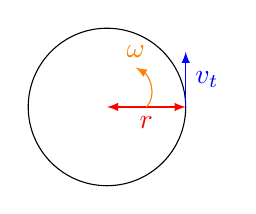
\begin{tikzpicture}
		\draw (0,0) circle (1);
		\draw[latex-latex, red] (0,0) -- (1,0)
			node[pos=0.5, below]{$r$};
		\draw[-latex, blue] (1,0) -- (1, 0.7)
			node[pos=0.5, right]{$v_t$};
		\draw[-latex, orange] (0.5,0) to[out=45, in=-30] (0.366, 0.5)
			node[above]{$\omega$};
	\end{tikzpicture}
\end{center}
Nel moto circolare, si distinguono due generi diversi di velocità: \emph{tangenziale} e\
\emph{angolare}.\\[\baselineskip]
La velocità tangenziale ($\mathcolor{blue}{v_t}$) è quella che cambia ad ogni istante direzione e che varia in base alla distanza dal centro.\\
La velocità angolare ($\mathcolor{orange}{\omega}$) è costante per ogni punto della circonferenza e 
indica quanto veloce un corpo ruota.\\[\baselineskip]
Si noti anche che $\mathcolor{red}{r}$ indica la distanza dal centro di rotazione al corpo in oggetto.
\\[\baselineskip]
\textbf{Velocità tangenziale}
\begin{equation*}
\mathcolor{blue}{v_t} = \frac{2\pi\mathcolor{red}{r}}{T} =
\mathcolor{orange}{\omega}\mathcolor{red}{r}
\end{equation*}
$r$: raggio della circonferenza\\
$T$: periodo del moto, ovvero quanto impiega a compiere un giro completo\\
$\mathcolor{orange}{\omega}$: velocità angolare

\textbf{Velocità angolare}
\begin{equation*}
\mathcolor{orange}{\omega} = \frac{\alpha}{t} = \frac{2\pi}{T}
\end{equation*}
$\alpha$: angolo percorso\\ 
$t$: tempo\\
$T$: periodo del moto

\textbf{Accelerazione centrifuga}
\begin{equation*}
a_c = \frac{\Delta \mathcolor{blue}{v}}{T} = \frac{2\pi\mathcolor{orange}{\omega}}{T} = 
\mathcolor{orange}{\omega}^2\mathcolor{red}{r} = \frac{\mathcolor{blue}{v}^2}{\mathcolor{red}{r}} = 
\mathcolor{orange}{\omega}\mathcolor{blue}{v}
\end{equation*}
$\Delta\mathcolor{blue}{v}$: variazione di velocità\\
$T$: periodo del moto\\
$\mathcolor{orange}{\omega}$: velocità angolare\\
$\mathcolor{red}{r}$: raggio della circonferenza

\subsection{Moto Armonico}
Il moto armonico è periodico, ovvero posizione, velocità e accelerazione si ripetono a intervalli 
regolari. Un esempio chiaro di moto armonico è il pendolo.\\
Molte delle formule del moto armonico sono ricavabili dal moto circolare.
\begin{equation*}
x = \mathcolor{red}{r}\sin\mathcolor{orange}{\omega}t
\end{equation*}
\begin{equation*}
\vec{a} = -\mathcolor{orange}{\omega}\vec{x}
\end{equation*}
$\mathcolor{red}{r}$: raggio della circonferenza\\
$\mathcolor{orange}{\omega}$: velocità angolare\\
$x$: posizione dell'oggetto\\
$\alpha$: accelerazion angolare

\subsection{Moto Circolare Uniformemente Accelerato}\label{subsec:cinematica:mrua}
\label{subsec:mrua}
È un moto circolare avente accelerazione costante in modulo.
\begin{equation*}
\theta = \theta_0 + \mathcolor{orange}{\omega}t
\end{equation*}
\begin{equation*}
\mathcolor{orange}{\omega} = \omega_0 + \alpha t
\end{equation*}
\begin{equation*}
\theta = \theta_0 + \omega_0t + \frac{1}{2}\alpha t
\end{equation*}
\begin{equation*}
a_t = \alpha \mathcolor{red}{r}
\end{equation*}
$\theta$: posizione angolare\\
$\mathcolor{orange}{\omega}$: velocità angolare\\
$\mathcolor{red}{r}$: raggio della circonferenza\\
$t$: tempo\\
$a_t$: accelerazione tangenziale\\
$\alpha$: accelerazione angolare
